\documentclass[tikz,border=4pt]{standalone}
\usepackage{amsmath}
\begin{document}
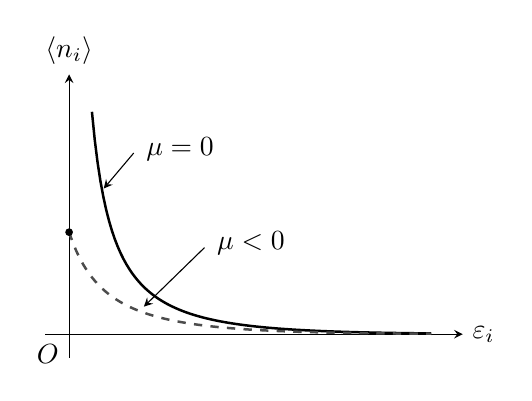
\begin{tikzpicture}[>=stealth, thick, scale=1.0]
  % Axes
  \draw[->, line width=0.4pt] (-0.3, 0) -- (5.0, 0) node[right] {$\varepsilon_i$};
  \draw[->, line width=0.4pt] (0, -0.3) -- (0, 3.3) node[above] {$\langle n_i \rangle$};
  \node[below left] at (0, 0) {$O$};

  % mu = 0 (solid, diverges as eps_i -> +0)
  \draw[line width=0.9pt, domain=0.29:4.6, samples=120]
    plot (\x, {0.95 / (exp(\x) - 1)});

  % mu < 0 (dashed, finite at eps_i = 0)
  \draw[dashed, line width=0.9pt, black!70, domain=0:4.6, samples=100]
    plot (\x, {0.95 / (exp(\x + 0.55) - 1)});
  \fill (0, {0.95/(exp(0.55)-1)}) circle (1.4pt);

  % Labels
  \node[right] at (0.85, 2.35) {$\mu = 0$};
  \draw[->, line width=0.4pt] (0.82, 2.3) -- (0.44, 1.85);

  \node[right] at (1.75, 1.15) {$\mu < 0$};
  \draw[->, line width=0.4pt] (1.72, 1.1) -- (0.95, 0.35);
\end{tikzpicture}
\end{document}
